\label{chapter:resultados}

Este capítulo tem como objetivo apresentar o planejamento, execução e análise dos resultados obtidos a partir implementação do método proposto no sistema Hand.io. Esta avaliação teve como foco o funcionamento do protótipo da luva por meio de experimentações em cenários reais levando em consideração a eficácia e a eficiência do sistema em situações de utilização normal.

\section{Análise da implementação}

Nesta seção é detalhado e analisado de maneira extensiva as particularidades da implementação da Hand.io, tanto no projeto do \textit{hardware} quanto de \textit{software}.
% 
% \subsection{Análise do protótipo}
% 
Como definido no método proposto no \autoref{chapter:metodo}, o protótipo da Hand.io consiste em duas partes: a luva de captura de movimentos e a central de processamento de sinais que controla os dispositivos. Ambas as partes serão avaliadas de forma individual nas seções a seguir.

\subsection{Protótipo da luva de captura de movimentos}

A luva é composta por três principais componentes: 
microcontrolador Arduino UNO, que decodifica os sinais do sensor e os envia pela porta serial conectada à central de processamento (Figura~\ref{fig:dorso}); 
um sensor MPU $6050$, composto por um acelerômetro e um giroscópio, que é utilizado para realizar a leitura dos movimentos (Figura~\ref{fig:dorso}); e 
um botão, acionado pelo usuário para definir o início e o fim da captura dos movimentos (Figura~\ref{fig:palma}). Os três componentes podem ser vistos na \autoref{fig:luva}.

\begin{figure}[ht]
    \centering
    \caption{Projeto da luva.}
    \subfloat[\label{fig:dorso}]
        {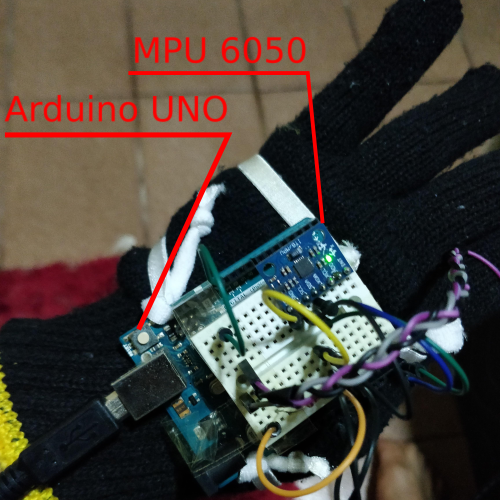
\includegraphics[width=0.39\textwidth]{resources/luva1.png}}
        \hspace{0.5cm}
    \subfloat[\label{fig:palma}]
        {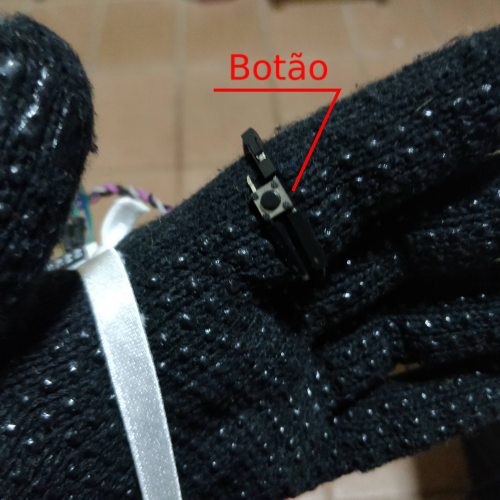
\includegraphics[width=0.39\textwidth]{resources/luva2.png}}
    \legend{Fonte: Elaborada pelo autor.}
    \label{fig:luva}
\end{figure}

% Os componentes estão posicionados de maneira a garantir o máximo de conforto possível ao usuário. 
% É recomendada a utilização de 
Neste protótipo adotou-se uma luva de pano para reduzir o contato do Arduino com a pele.
% , pois os pontos de solda no verso da placa podem criar eventuais escoriações com a utilização prolongada do sistema. 
O Arduino foi posicionado no dorso da mão de maneira firme, com fitas elásticas para evitar movimentações indesejadas que levariam à uma leitura imprecisa dos movimentos.
% 
O sensor MPU $6050$ está fixado em uma \textit{mini protoboard} presa no topo do Arduino com fitas adesivas de maneira estável. O botão de acionamento de captura de movimentos conta com os seus fios trançados, a fim aumentar a rigidez da construção do protótipo. Ao final da trança os fios são ligados ao botão de modo a formar um anel em volta do dedo indicador do usuário. Este posicionamento visa aumentar a ergonomia da luva, pois o botão estará convenientemente localizado no alcance do polegar do operador.

\subsection{Protótipo da central de processamento de sinais}
\label{sec:prototipo}
O esquemático da central apresentado na \autoref{fig:esq_central} do \autoref{chapter:metodo} define que a central é composta por um computador de propósito geral equipado com um microprocessador, capaz de executar algoritmos de aprendizado de máquina e enviar e receber sinais infravermelhos. Componentes com as mesmas funcionalidades dos propostos inicialmente no método foram utilizados no protótipo final, de maneira que foi possível validar o método proposto sem que fossem realizadas mudanças significativas.

\begin{figure}[ht]
    \centering
    \caption{Central de controle.}
    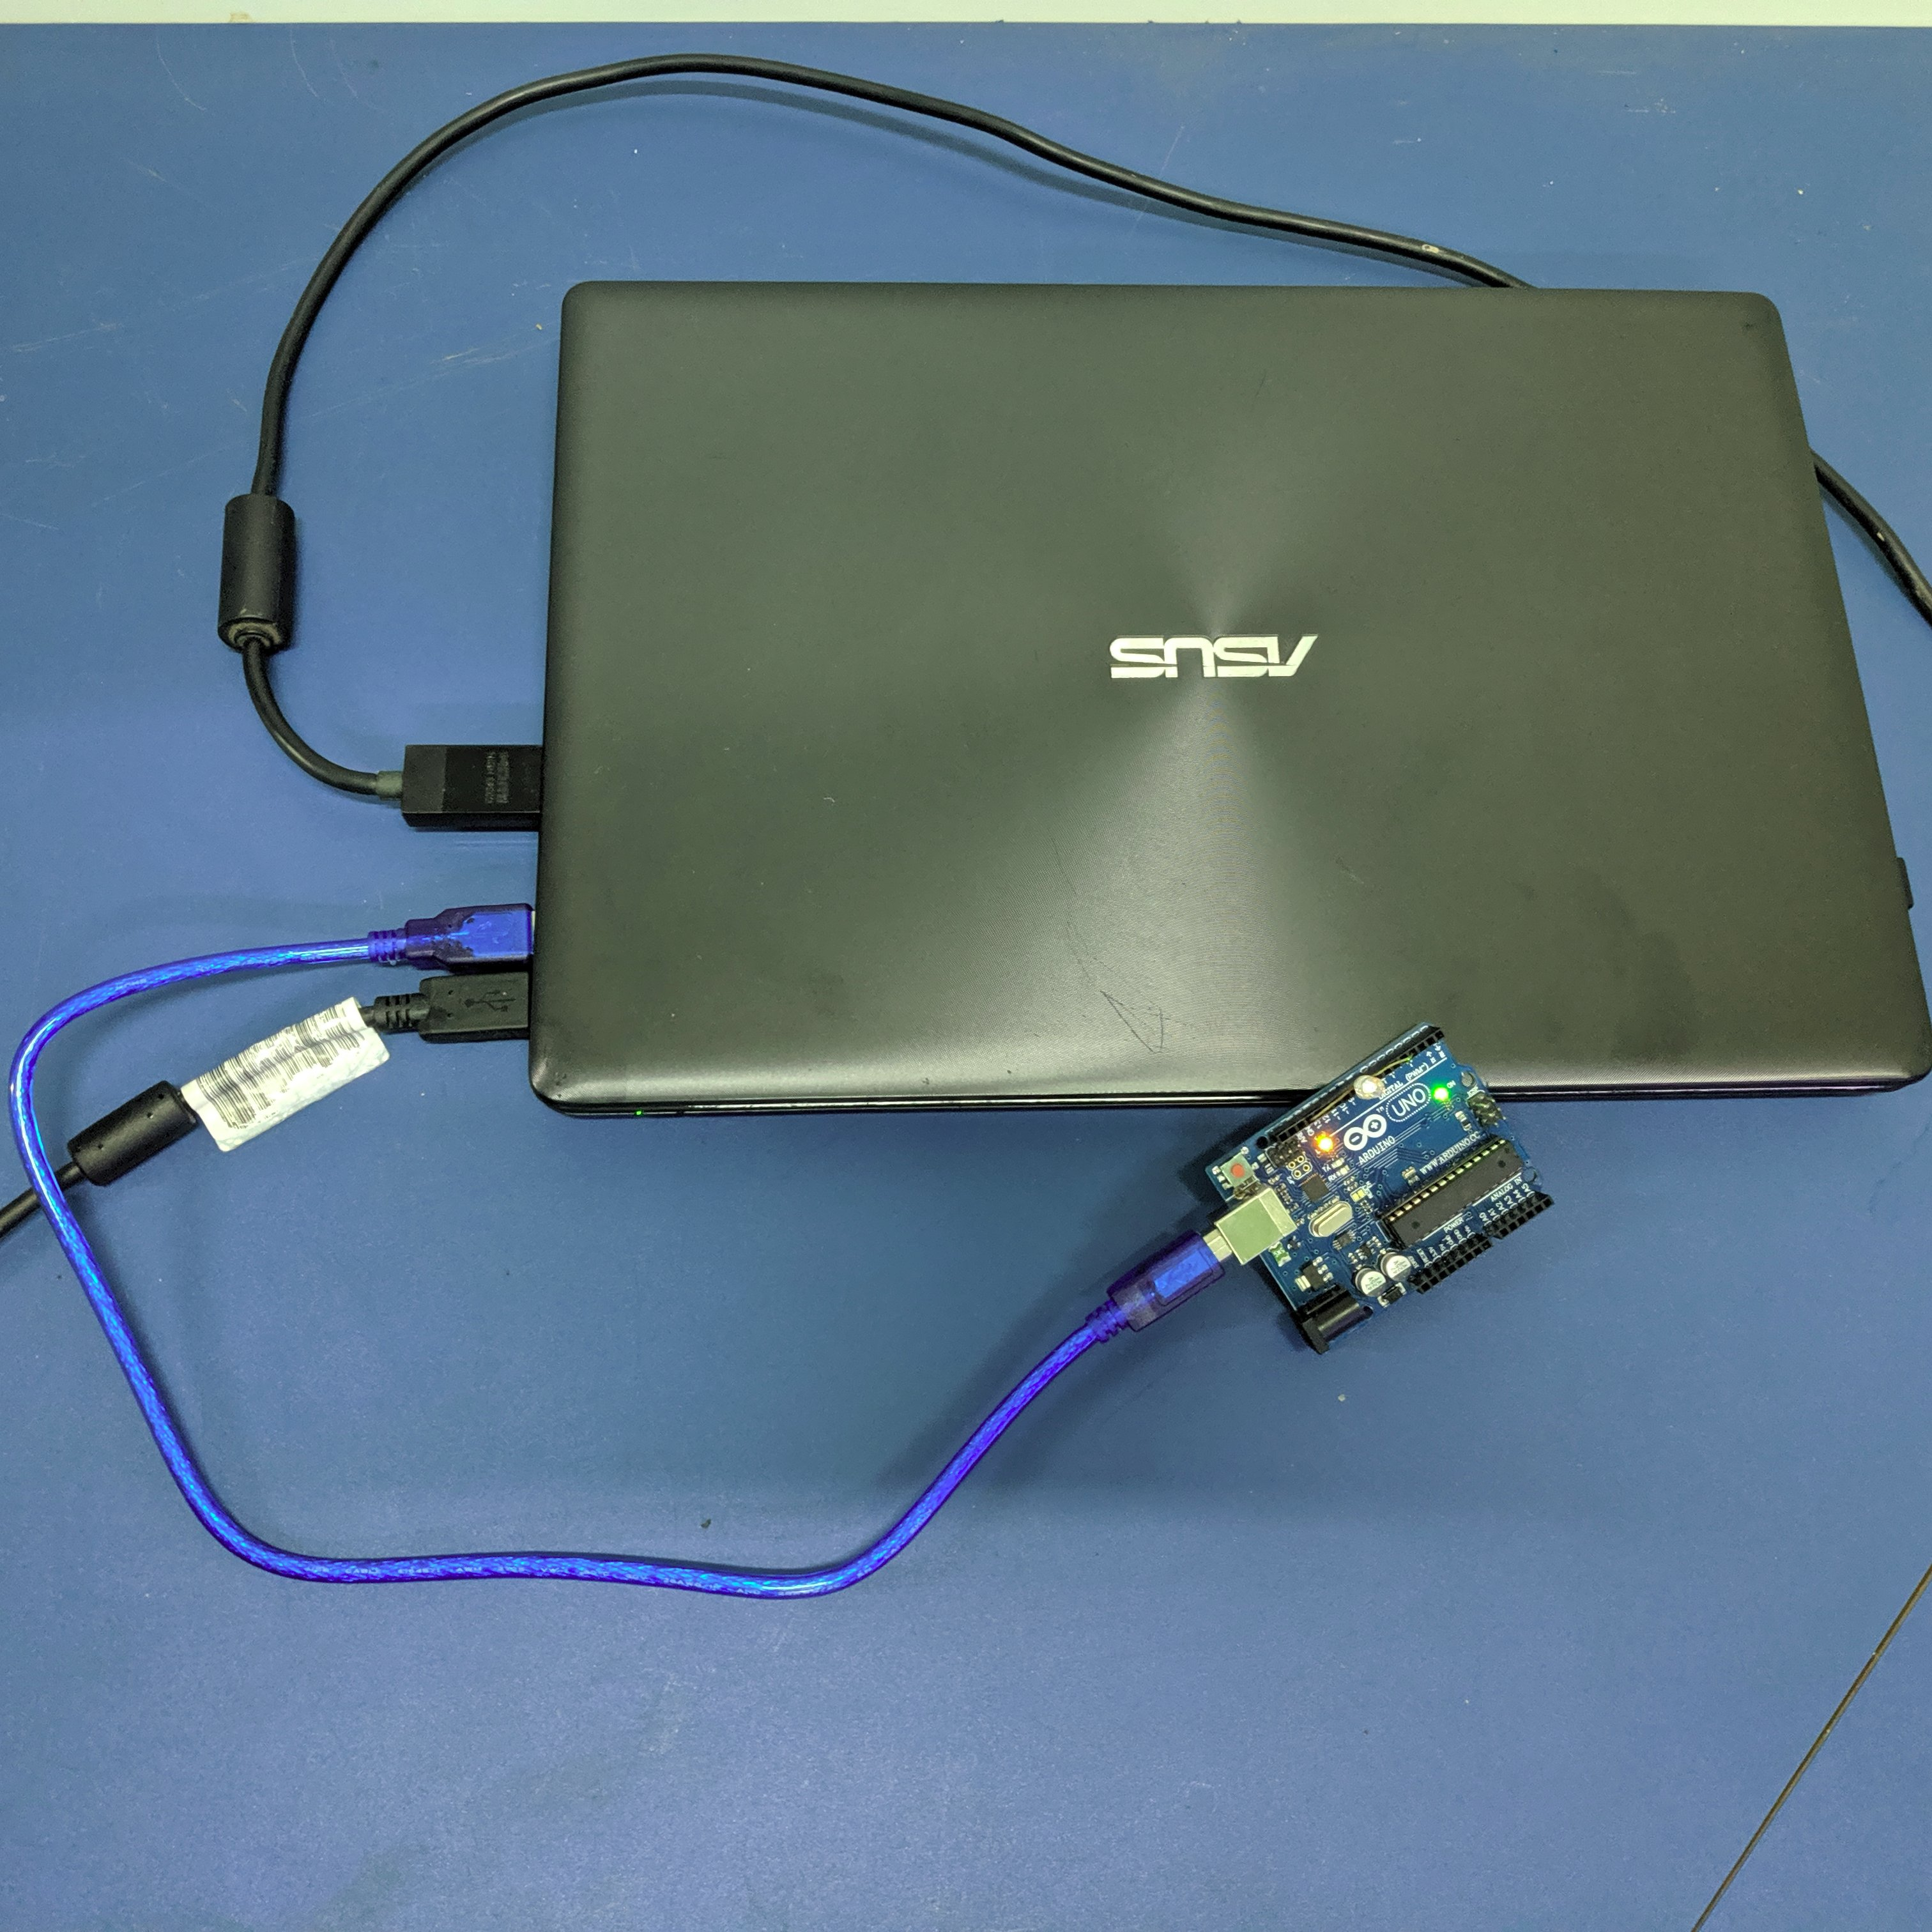
\includegraphics[width=0.5\textwidth, keepaspectratio]{resources/central.jpg}
    \legend{Fonte: Elaborada pelo autor.}
    \label{fig:central}
\end{figure}

O protótipo da central exibido na \autoref{fig:central}, é composto por um Notebook Asus com um processador \textit{Intel Core I5}, $6GB$ de memória \textit{RAM}, rodando o sistema operacional Manjaro Linux 18.0.4, conectado à luva através de uma conexão serial via cabo por uma porta USB, que processa os sinais recebidos e executa as ações correspondentes. Através de uma outra porta USB do Notebook, uma outra conexão serial ligada à um segundo Arduino UNO como atuador, é realizada. Este Arduino é a interface para emissão e recepção de sinais infravermelhos para o controle de dispositivos no ambiente. 
% É recomendado que o atuador fique em um lugar próximo aos dispositivos que se deseja controlar devido ao alcance limitado do emissor de infravermelho.



\subsection{Análise do software do protótipo Hand.io}

O sistema é composto por três softwares que estão sendo executados simultaneamente de maneira independente no protótipo. Um no Arduino acoplado à luva, um no Arduino conectado à central e um na central de processamento. O código-fonte deste projeto está disponível no repositório online GitHub \url{https://github.com/JohnPinto/Hand.io}.

\subsubsection{Análise dos softwares embarcados nos Arduinos}

Os softwares em execução nos dois Arduinos funcionam de maneira distinta. Durante a modelagem do sistema, foi definido que o Arduino presente na luva funcionaria apenas como sensor, enviando os sinais dos movimentos para a central, enquanto o encontrado na central serviria de atuador, enviando os sinais infravermelhos para os dispositivos a serem controlados.

No decorrer do funcionamento normal do sistema o Arduíno embutido na luva lê os sinais do sensor em tempo real. Enquanto o botão de captura de movimentos presente na luva não for pressionado pelo usuário, é enviado para a central apenas uma sequência de pontos (\texttt{.}) com um intervalo de 5ms entre os envios. 

O comportamento, de envio intercalado de pontos (\texttt{.}) e sinais de movimento, serve de condição de marca parada para o classificador de movimentos encontrado na central que será detalhado nas seções a seguir. Foi utilizada a biblioteca SoftwareSerial\footnote{\url{https://www.arduino.cc/en/Reference/SoftwareSerial}\label{ftnote:serial}} para a realização de comunicação serial.

Quando o botão na luva é pressionado, o sensor passa a enviar, o sinal do acelerômetro e do giroscópio, pela porta serial, formatado  seguindo o padrão, representado na sequência de caractesres \texttt{\$    ax    ay    az    gx    gy    gz    $\setminus $n}, onde as componentes \texttt{x, y} e \texttt{z} dos sensores são indicadas pelas letras \texttt{a} para acelerômetro e \texttt{g} para giroscópio, o \texttt{\$}, indica o início da leitura e o \texttt{$\setminus $n}, uma quebra de linha, indica o fim. 

% O sinal é enviado desta maneira afim de garantir a consistência da transmissão dos dados. 

O Arduino conectado à central que serve de atuador, permanece ocioso até que um comando indicando qual sinal infravermelho deverá ser enviado seja recebido. Os códigos infravermelhos ficam armazenados diretamente no Arduino, em função do desacoplamento dos códigos da memória RAM para a flash\footnote{\url{https://www.arduino.cc/reference/en/language/variables/utilities/progmem/}}, isto permite ao usuário realizar o cadastro de centenas de códigos infravermelhos de dispositivos diferentes. 

Devido à natureza estacionária da central, é possível que múltiplos atuadores estejam inseridos em diversos cômodos diferentes de uma casa, por exemplo, o que serviria de aplicação para este trabalho. Na implementação deste software foram utilizadas as bibliotecas SoftwareSerial\textsuperscript{\ref{ftnote:serial}}, para comunicação serial, e IRremote\footnote{\url{https://github.com/z3t0/Arduino-IRremote}}, para envio de sinais infravermelhos a partir do Arduino.


\subsubsection{Análise do software da central de processamento}


O software em execução na central de processamento tem a implementação detalhada na \autoref{fig:class}, onde é apresentado o diagrama de classes que define as especificidades do sistema e detalha as relações entre as classes que o constituem.

\begin{figure}[ht]
    \centering
    \caption{Diagrama de classe da Hand.io.}
    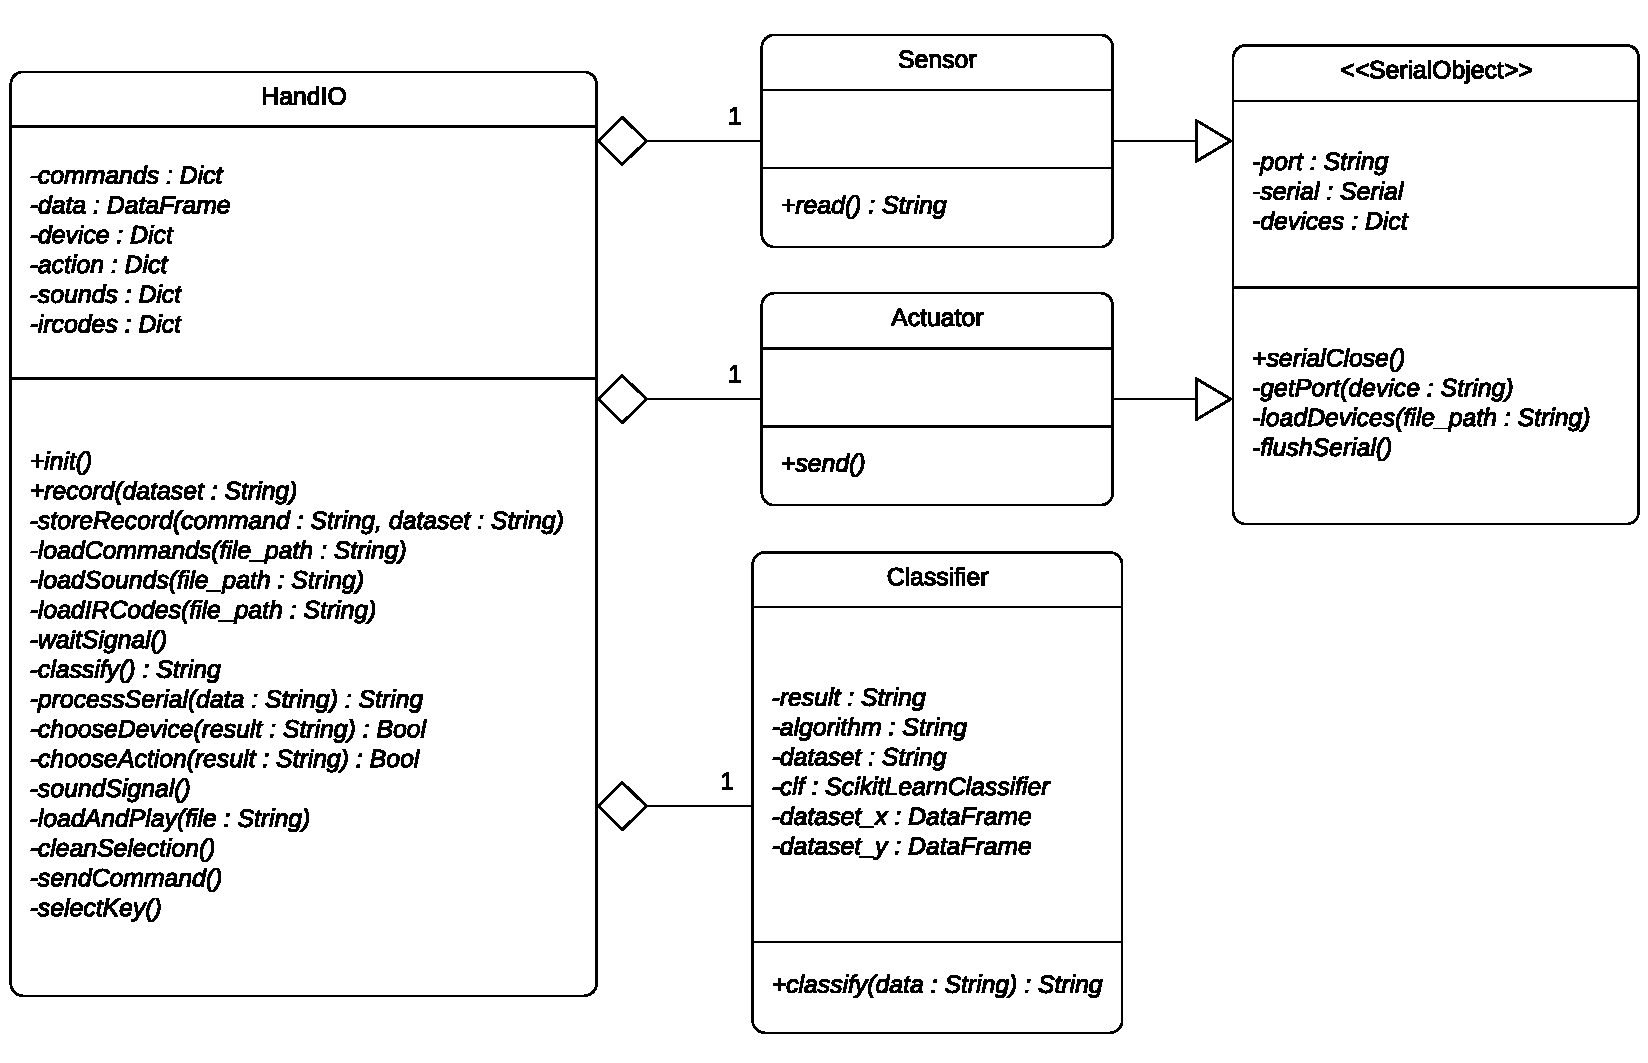
\includegraphics[width=\textwidth, keepaspectratio]{resources/diagrama_classe.pdf}
    \legend{Fonte: Elaborada pelo autor.}
    \label{fig:class}
\end{figure}

O código-fonte foi desenvolvido na linguagem de programação Python $3$, utilizando conceitos de programação orientada a objetos, como classes e herança, visando compartimentalizar o código com o objetivo de aumentar a previsibilidade, e evitar retrabalhos por parte do desenvolvedor. 

A linguagem em questão foi escolhida por sua praticidade de implementação por causa da sua natureza de alto nível, o que permite uma implementação rápida e simples em comparação com as demais linguagens. Outro fator motivador é a presença de uma vasta gama de bibliotecas externas que agilizaram o desenvolvimento do protótipo, como o Scikit-learn\footnote{\url{https://scikit-learn.org/}\label{ftnote:sklearn}}
% , que dispõe de biblioteca Scikit-learn 
que conta com uma série de classificadores que utilizam algoritmos de aprendizado de máquina já implementados, e a PySerial\footnote{\url{https://github.com/pyserial/pyserial}\label{ftnote:pyserial}} que reliza o interfaceamento entre a linguagem Python e as portas seriais que conectam o sistema àos sensores e atuadores.

No diagrama de classes da \autoref{fig:class} a \texttt{HandIO} é a classe principal do sistema. Esta classe conta com definições de sensor, atuador e classificador. Ambos, os sensores e atuadores, implementados nas classes de nomes correspondentes, herdam da classe abstrata \texttt{SerialObject}, com a diferença de que o sensor tem a capacidade de enviar sinais e o atuador apenas de recebe-los. Internamente a classe \texttt{SerialObject} utiliza a biblioteca PySerial, para a transmissão de dados. 

A classe \texttt{HandIO} conta com diversos dicionários que agem como uma especie de banco de dados do sistema, esta abordagem foi escolhida para que haja a possibilidade do desenvolvedor do sistema modificar ou adicionar novos gestos ou dispositivos de maneira simplificada. Todos os dicionários utilizados são carregados a partir de seus arquivos \texttt{.json} correspondentes que podem ser encontrados na pasta \texttt{json/} da raiz do sistema. Foram implementados métodos privados que iniciam com a palavra \texttt{load}, que carregam cada dicionário individualmente, estes métodos são chamados no construtor do objeto.

O classificador, implementado na classe \texttt{Classifier}, utiliza a biblioteca Scikit-learn. Esta biblioteca foi escolhida por suprir as necessidades do protótipo, e contar com uma \texttt{API} de utilização bastante simplificada. Os datasets com registros de movimentos utilizados para geração do modelo de classificação dos gestos ficam armazenados na pasta \texttt{datasets/} do programa. 

A geração destes datasets se dá utilizando o método público \texttt{record()} da classe \texttt{HandIO}, que pede que o usuário da luva insira uma classe, que define qual gesto será registrado, e realize a captura de $10$ gestos. Este procedimento se repete até que o usuário pare o programa. Para o protótipo foi levantado um \texttt{dataset} com $360$ leituras recolhidas de nove voluntários diferentes, distribuídas entre quatro classes de gestos correspondentes à movimentos nas direções cima, baixo, direita e esquerda. Os voluntários foram orientados a realizar os gestos com a palma da mão voltada para a direita. Estes gestos foram escolhidos devido ao seu baixo grau de complexidade o que facilitaria os experimentos detalhados nas seções seguintes.

Para a definição de qual classificador seria o mais eficaz para a classificação de gestos, foi realizado um comparativo, com os principais classificadores oferecidos pela biblioteca Scikit-learn, sendo estes: a \textit{Logistic Regression} (LR)~\cite{scikit:lr}, a \textit{Linear Discriminant Analysis} (LDA)~\cite{scikit:lda}, o \textit{K-Neighbors Classifier} (KNN)~\cite{scikit:knn}, o \textit{Decision Tree Classifier} (CART)~\cite{scikit:cart}, a \textit{Gaussian Naive Bayes} (NB)~\cite{scikit:nb}, a \textit{Suport Vector Machine} (SVM)~\cite{scikit:svm}, o \textit{Ada Boost Classifier} (ADB)~\cite{scikit:adb}, o \textit{Random Forest Classifier} (RFC)~\cite{scikit:rfc}, o \textit{Extra Trees Classifier} (ETC)~\cite{scikit:etc}, e o \textit{Gradient Boosting Classifier} (GBC)~\cite{scikit:gbc}.

Este comparativo foi realizado utilizando validação cruzada~\cite{scikit:crossval}, técnica que divide o dataset em grupos de treinamento e grupos de teste. O grupo de treinamento é utilizado para a criação do modelo de classificação que serve de referência para classificações futuras, e o grupo de testes é utilizado como entrada para o classificador, esperando que a classificação seja bem sucedida, já que ambas as partes fazem parte de um mesmo dataset. Para uma medição mais precisa foi utilizada a técnica conhecida como $K$-fold~\cite{scikit:crossval}, que realiza $K$ testes de validação cruzada pegando $K$ partes, como treinamento e teste, a cada $K$ interações. Para a obtenção de resultados consistentes foi utilizado um $K = 10$.

Após a execução do comparativo, os resultados constatados na \autoref{tab:comparativo}, indicam que o classificador com melhor desempenho foi o \textit{Gaussian Naive Bayes} (NB), que obteve uma acurácia de 81.1\% durante a validação cruzada, sem que houvesse uma perda considerável na pontuação de treino no decorrer do aumento da quantidade de registros de movimento no \textit{dataset}.

\begin{table}[ht]
    \centering
    \caption{Comparativo dos classificadores.}
    \begin{tabular}{cccccc}
        \hline
        \multicolumn{1}{|c|}{\textbf{Classificador}} & \multicolumn{1}{c|}{\textbf{LR}} & \multicolumn{1}{c|}{\textbf{LDA}} & \multicolumn{1}{c|}{\textbf{KNN}} & \multicolumn{1}{c|}{\textbf{CART}} & \multicolumn{1}{c|}{\textbf{NB}} \\ \hline
        \multicolumn{1}{|c|}{\textbf{Acurácia}} & \multicolumn{1}{c|}{62.7\%} & \multicolumn{1}{c|}{73.8\%} & \multicolumn{1}{c|}{77.5\%} & \multicolumn{1}{c|}{71.3\%} & \multicolumn{1}{c|}{81.1\%} \\ \hline
        \multicolumn{1}{l}{} & \multicolumn{1}{l}{} & \multicolumn{1}{l}{} & \multicolumn{1}{l}{} & \multicolumn{1}{l}{} & \multicolumn{1}{l}{} \\ \hline
        \multicolumn{1}{|l|}{\textbf{Classificador}} & \multicolumn{1}{c|}{\textbf{SVM}} & \multicolumn{1}{c|}{\textbf{ADB}} & \multicolumn{1}{c|}{\textbf{RFC}} & \multicolumn{1}{c|}{\textbf{ETC}} & \multicolumn{1}{c|}{\textbf{GBC}} \\ \hline
        \multicolumn{1}{|c|}{\textbf{Acurácia}} & \multicolumn{1}{c|}{79.7\%} & \multicolumn{1}{c|}{49.1\%} & \multicolumn{1}{c|}{77.7\%} & \multicolumn{1}{c|}{78.8\%} & \multicolumn{1}{c|}{74.1\%} \\ \hline
    \end{tabular}
    \legend{Fonte: Elaborada pelo autor.}
    \label{tab:comparativo}
\end{table}

\begin{figure}[ht]
    \centering
    \caption{Classificador Gaussian Naive Bayes.}
    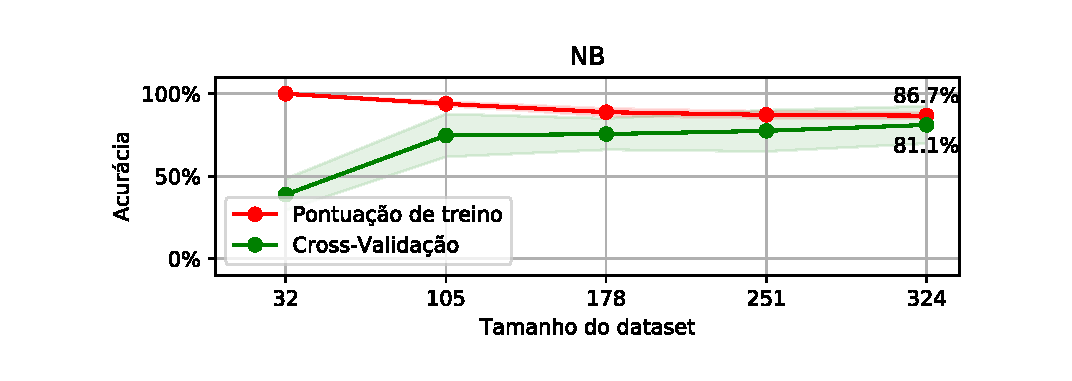
\includegraphics[width=0.9\textwidth, keepaspectratio]{resources/comparacao.pdf}
    \legend{Fonte: Elaborada pelo autor.}
    \label{fig:naivebayes}
\end{figure}

Apesar do gráfico do NB, apresentado na \autoref{fig:naivebayes}, com $32$ valores valores no \textit{dataset} ter atingido uma pontuação de treino alta em relação à uma quantidade maior, o modelo gerado com apenas esta quantidade de valores não é genérico o suficiente para classificar os movimentos de um segundo usuário com precisão, por isso é necessária uma quantidade maior de leituras realizadas por usuários diferentes, o que justifica a escolha deste classificador como o classificador padrão deste sistema.

\subsection{Fluxo de execução do Hand.io}

O sistema conta com duas grandes fases apresentadas na máquina de estados da \autoref{fig:automato}. A fase de seleção de dispositivo, definida na parte superior da figura, e a fase de seleção de ação, na parte inferior. O fluxo de execução será abordado do ponto de vista da máquina de estados, realizando anotações sobre quais métodos das classes, expostos na \autoref{fig:class}, são chamados durante um dado estado. 
% 
Na classe \texttt{HandIO} está implementado o método público \texttt{init()}, que é responsável pelo funcionamento nominal da central. Os procedimentos dentro deste método, refletem o comportamento definido na máquina de estados apresentada anteriormente.

\begin{figure}[ht]
    \centering
    \caption{Máquina de estados da Hand.io.}
    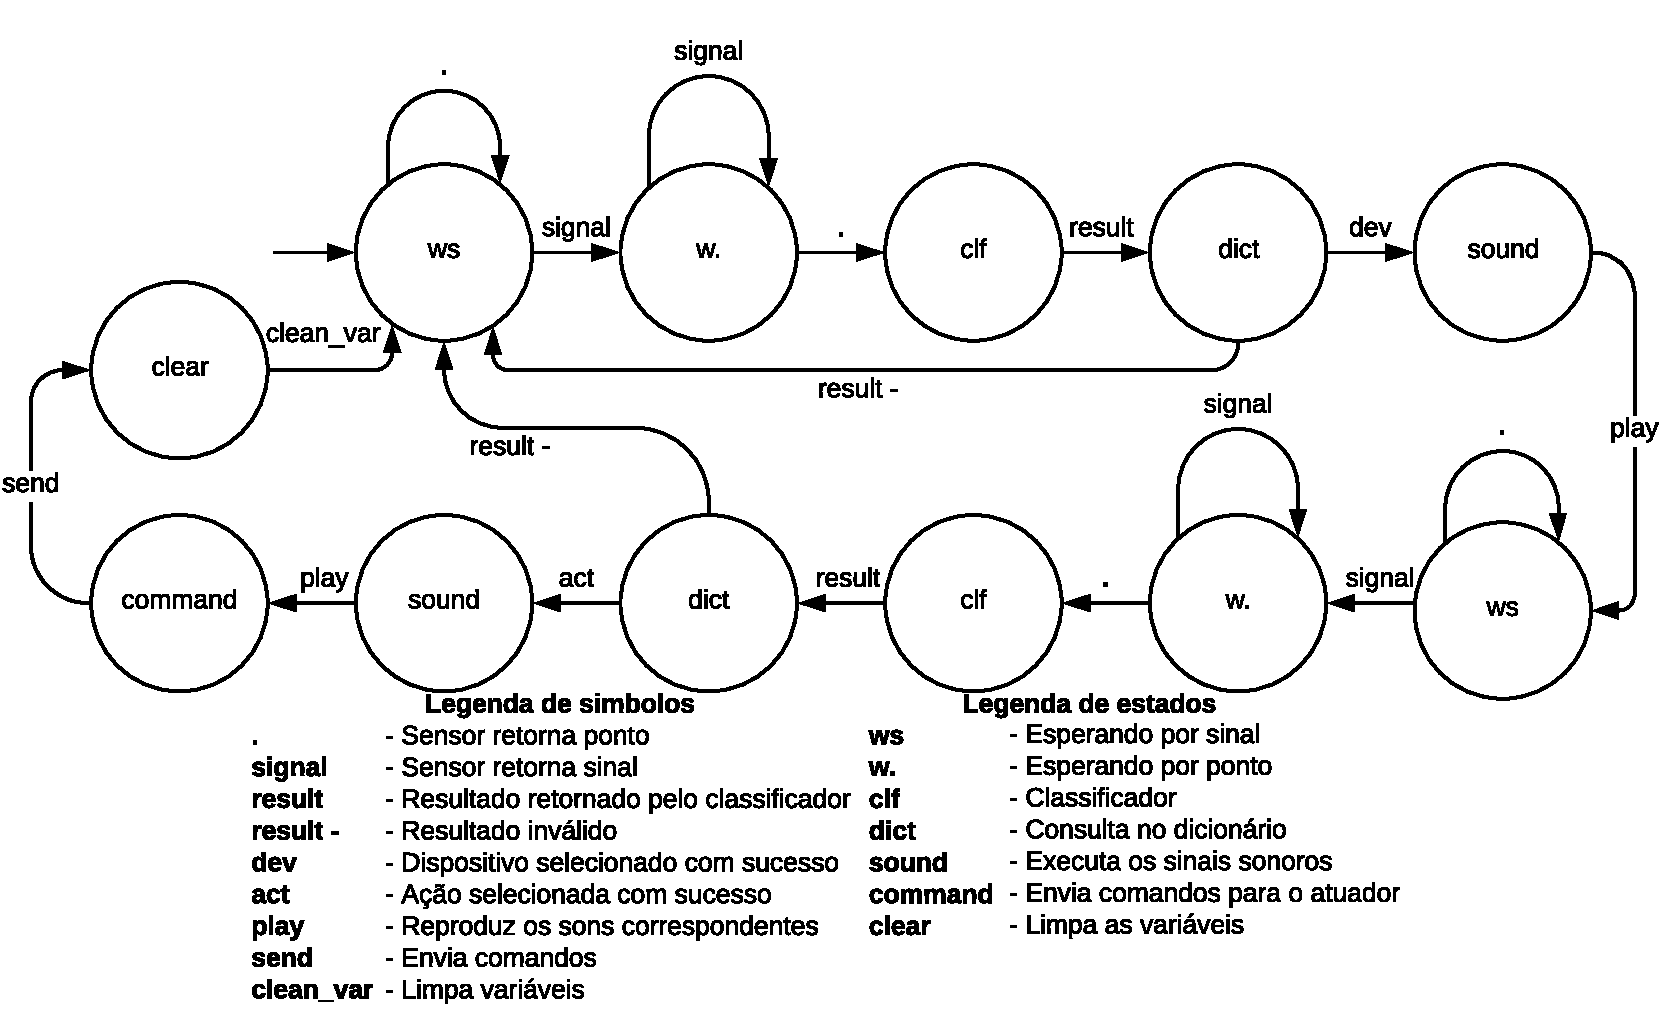
\includegraphics[width=\textwidth, keepaspectratio]{resources/maquina_estados.pdf}
    \legend{Fonte: Elaborada pelo autor.}
    \label{fig:automato}
\end{figure}

Durante os estágios iniciais da primeira e da segunda fase, os estados \textbf{ws} e \textbf{w.}, que foram implementados no método \texttt{waitSignal()}, o sistema fica aguardando os sinais de início e parada de captura de movimentos. Em um primeiro momento, ao receber pontos pela serial, a central permanece no estado \textbf{ws}, quando for constatado o recebimento de um sinal de movimento, o sistema passará para o estado \textbf{w.}.

O programa permanecerá neste estado até que voltem a ser recebidos pontos, para que, então, o ultimo sinal recebido seja salvo no atributo \texttt{data}, e enviado para o classificador no estado \textbf{clf} que chama o método \texttt{classify()}. Após o retorno da classificação, o sistema passará para o estado \textbf{dict}, onde os resultados serão avaliados.

Neste estado o resultado da classificação serve como entrada para o método \texttt{chooseDevice()} ou para o método \texttt{chooseAction()}, dependendo da fase que o programa se encontra. Nestes métodos o resultado é utilizado como chave no dicionario \textit{commands} que retorna o dispositivo ou ação correspondente ao gesto. 
Caso o dicionário retorne um sinal válido o sistema então passa para o estado \textbf{sound}, que chama o método \texttt{soundSignal()} caso o retorno seja inválido o sistema retornará ao estado inicial. Durante a segunda fase do programa os possíveis retornos do dicionário ficam restritos às possíveis ações que dispositivo previamente selecionado tem mapeados pelo sistema. 

O estado \textbf{command}, implementado no método \texttt{sendCommand()}, analisa a ação selecionada no estado anterior e as realiza no dispositivo selecionado. Ao final das duas fases o sistema entra no estado \textbf{clear}, que limpa a seleção de dispositivo e gesto, para que um novo comando seja realizado. 

\section{Planejamento e projeto do cenário experimental}

Um cenário, no qual serão realizados os experimentos, foi criado para avaliar a capacidade da Hand.io de controlar dispositivos em um ambiente real. Será utilizado, nesta avaliação, o protótipo discutido na seção anterior deste capítulo. Como referência do progresso dos experimentos, as questões experimentais levantadas abaixo serão respondidas conforme o andamento dos experimentos:

\begin{description}
    \item [QE1] \label{qa:1} - Qual a taxa de sucesso do sistema Hand.io em detectar os gestos corretamente e enviar sinais aos dispositivos correspondentes?
    \item [QE2] \label{qa:2} - Um novo usuário do sistema Hand.io, usando um roteiro, consegue controlar os dispositivos de um dado ambiente?
    \item [QE3] \label{qa:3} - Qual a avaliação de um novo usuário sobre o estado atual do protótipo do sistema Hand.io?
\end{description}

O cenário experimental, apresentado na \autoref{fig:cenario}, conta com os seguintes dispositivos eletrônicos: um ar-condicionado, do fabricante Carrier de 36.000 \textit{BTU/h}; uma TV da marca Philips de 32 polegadas; e um software para apresentação de slides em um \textit{notebook}, definido na \autoref{sec:prototipo}. 
% , que serve de central para o sistema, e é exibida na TV. 
Para controle de dispositivos que contam com uma interface de controle por meio de sinais infravermelhos, como é o caso do ar-condicionado e da TV selecionas, é necessário que os sinais enviados pelos controles remotos destes dispositivos sejam capturados e carregados no Arduino que serve como atuador, no sistema Hand.io, esta etapa é feita durante o processo de instalação. 

Para controle da apresentação de slides, não é necessária intervenção por parte do instalador do sistema, pois o sistema já possui as funcionalidades para este tipo de operação, tendo os comandos do teclado que realizam o controle da apresentação já mapeados. O protótipo da Hand.io está localizado no alcance dos receptores infravermelhos dos dispositivos. O usuário que realizará os experimentos ficará em uma posição central no cenário.

\begin{figure}[ht]
    \centering
    \caption{Cenário experimental.}
    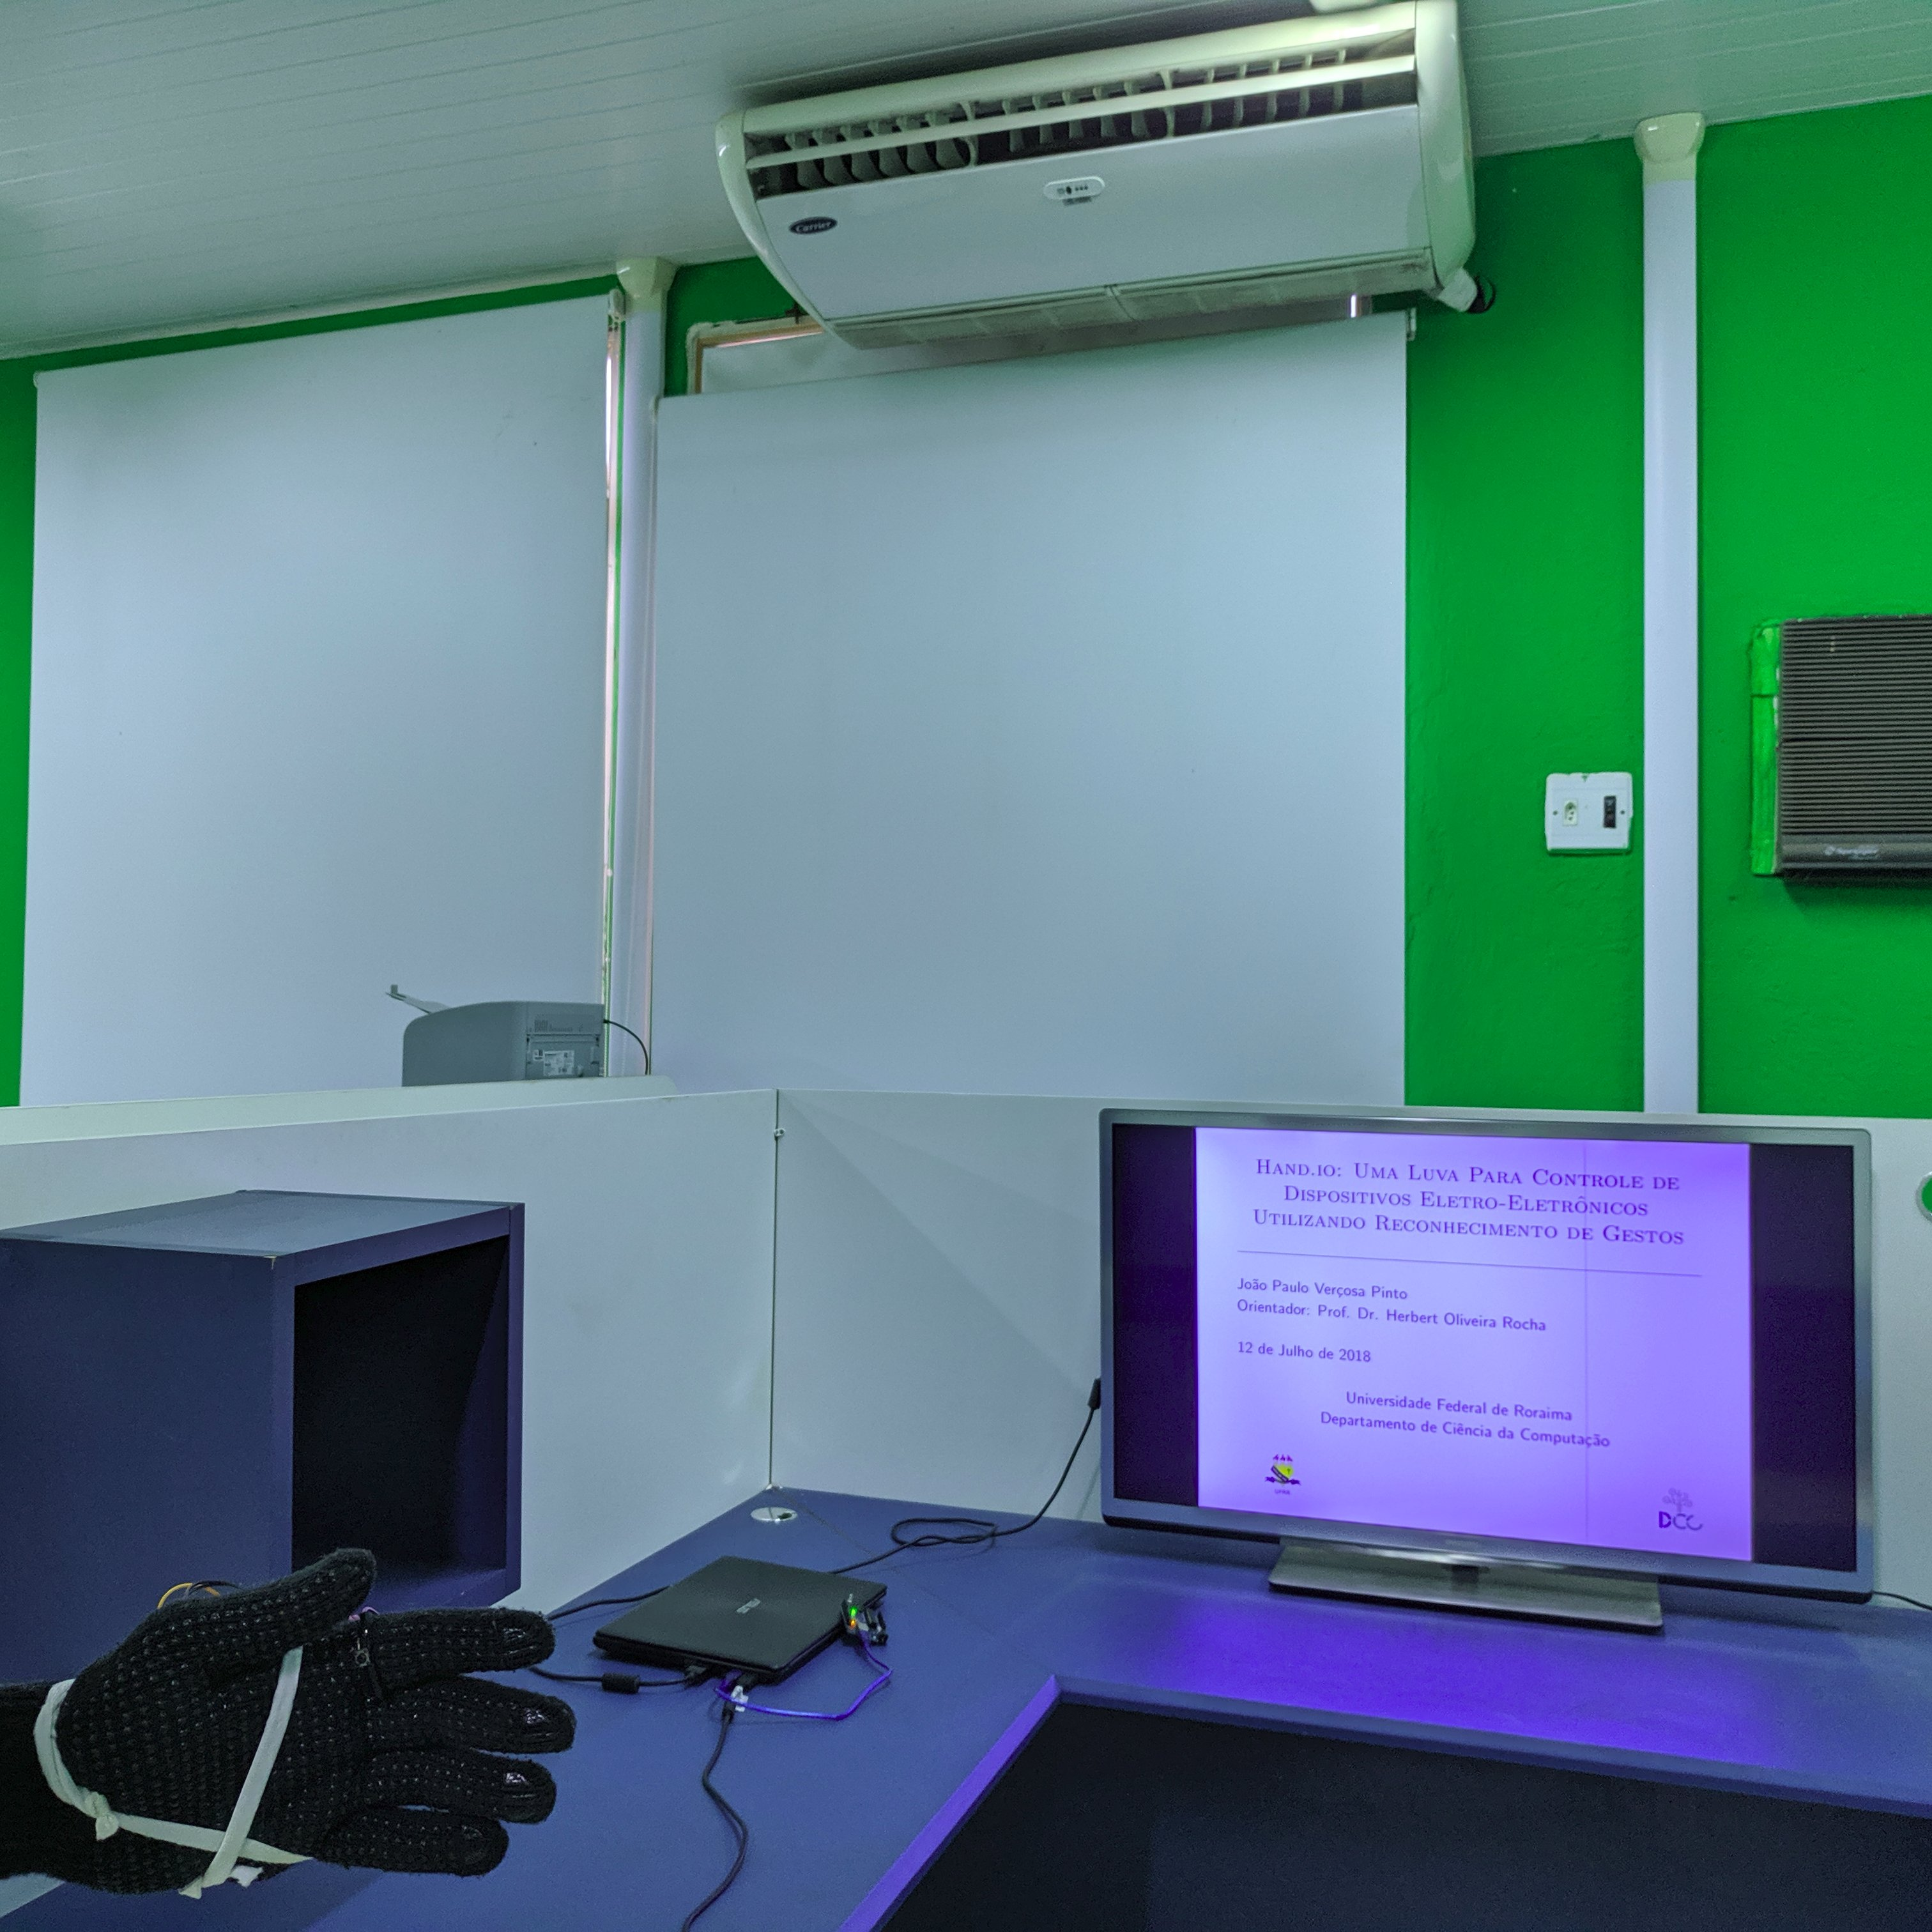
\includegraphics[width=0.5\textwidth, keepaspectratio]{resources/cenario.jpg}
    \legend{Fonte: Elaborada pelo autor.}
    \label{fig:cenario}
\end{figure}

Diante do proposto, foram realizados três experimentos, medindo a eficácia e execução do sistema proposto de maneiras diferentes. Com a finalidade de responder a primeira questão experimental (\textbf{QE1}), foi realizado um primeiro experimento onde um voluntário, que teve os seus dados de movimentos previamente cadastrados no sistema, reproduziu duas situações e teve a sua taxa de sucesso registrada quantitativamente.

Para a análise da segunda questão experimental (\textbf{QE2}), um grupo de voluntários, que nunca utilizou o sistema e não teve seus dados de movimentos previamente registrados, foi instruído a seguir um roteiro escrito de uso do Hand.io e teve a sua taxa de sucesso registrada para avaliação posterior. A descrição do experimento e seus resultados são apresentados na \autoref{Sect:ExecExperi}. 

O grupo anteriormente descrito foi utilizado em um outro experimento, a fim de responder a terceira questão experimental (\textbf{QE3}), após a execução do roteiro, os participante responderam um questionário, composto por perguntas sobre o estado atual do sistema proposto. Adicionalmente, foram coletadas sugestões dos participantes do experimento visando identificar quais possíveis melhorias poderiam ser feitas para a ergonomia do sistema a partir do ponto de vista de um eventual usuário final.

%\newpage

\section{Execução dos experimentos e análise dos resultados} \label{Sect:ExecExperi}

Durante está seção será detalhada a execução dos experimentos, e os seus resultados serão analisados com a finalidade de responder as questões experimentais levantas na seção anterior.

%\todo[inline]{Adicionar um texto de introduçao desta seção}

\subsection{Teste com um usuário experiente}

Após a execução do primeiro experimento, os resultados foram registrados e estão expostos na \autoref{tab:resultados}, onde a primeira coluna representa o número de vezes que o experimento proposto foi executado. A segunda e a terceira denotam os resultados das situações 1 e 2, respectivamente. Na situação 1, o usuário do Hand.io foi instruído a ligar e desligar sequencialmente a TV e o ar-condicionado presentes no cenário experimental. Já na situação 2, o usuário foi instruído a avançar ou retroceder a apresentação de slides reproduzida na TV. Cada resultado de um experimento $n$ está assinalado com um \textbf{OK}, para bem sucedido, e \textbf{F} para mal sucedido. 

\begin{table}[ht]
    \centering
    \caption{Dados coletados do experimento com um usuário experiente.}
    \resizebox{0.87\textwidth}{!}{
    \begin{tabular}{c|c|c|c|c|c|c|}
        \cline{2-7}
        & \multicolumn{4}{c|}{\textbf{Situação 1}} & \multicolumn{2}{c|}{\textbf{Situação 2}} \\ 
        \hline
        \multicolumn{1}{|c|}{$n$} & \textbf{Ligar TV} & \textbf{Ligar AC} & \textbf{Desligar TV} & \textbf{Desligar AC} & $\rightarrow$ & $\leftarrow$ \\
        \hline
        \multicolumn{1}{|c|}{\textbf{1}}  & OK & OK & OK & OK & OK & OK \\ \hline
        \multicolumn{1}{|c|}{\textbf{2}}  & OK & OK & OK & OK & OK & OK \\ \hline
        \multicolumn{1}{|c|}{\textbf{3}}  & OK & OK & OK & OK & OK & OK \\ \hline
        \multicolumn{1}{|c|}{\textbf{4}}  & OK & OK & OK & OK & OK & OK \\ \hline
        \multicolumn{1}{|c|}{\textbf{5}}  & OK & OK & OK & OK & OK & OK \\ \hline
        \multicolumn{1}{|c|}{\textbf{6}}  & OK & OK & OK & F  & OK & OK \\ \hline
        \multicolumn{1}{|c|}{\textbf{7}}  & OK & F  & OK & OK & OK & F  \\ \hline
        \multicolumn{1}{|c|}{\textbf{8}}  & OK & OK & OK & OK & OK & OK \\ \hline
        \multicolumn{1}{|c|}{\textbf{9}}  & OK & F  & OK & OK & OK & OK \\ \hline
        \multicolumn{1}{|c|}{\textbf{10}} & OK & OK & OK & OK & OK & OK \\ \hline
        \multicolumn{1}{|c|}{\begin{tabular}[c]{@{}c@{}}\textbf{Taxa}\\\textbf{de sucesso}\end{tabular}} & $100\%$ & $80\%$ & $100\%$ & $90\%$ & $100\%$ & $90\%$ \\ \hline
        \multicolumn{7}{|c|}{\textbf{Taxa média de sucesso:} $93.3\%$} \\ \hline
    \end{tabular}
    }
    \legend{Fonte: Elaborada pelo autor.}
    \label{tab:resultados}
\end{table}

A partir do total de 
% 60 experimentos, 
execuções do sistema distribuídos entre as situações $1$ e $2$, foi encontrada uma taxa média de sucesso de $93.3$\%, o que apresenta 
o funcionamento correto do sistema.
% de maneira evidente a eficácia do sistema. 
Apesar da taxa de falha ter sido pequena, ela não é desprezível em um sistema desenhado para um usuário final, logo se faz necessário um aprimoramento do classificador, a fim de reduzir ainda mais esse percentual. Os resultados apresentados por este experimentos servem de resposta para a questão experimental \textbf{QE1}.






%\newpage 

\subsection{Teste com voluntários inexperientes}

Um grupo com cinco voluntários que não tiveram contato anterior com o sistema, foi instruído a seguir um roteiro com a finalidade de avaliar a usabilidade e funcionamento da Hand.io. Os resultados deste experimento estão expostos na \autoref{tab:roteiro}, onde \textbf{V1}, \textbf{V2}, \textbf{V3}, \textbf{V4}, \textbf{V5} representam os voluntários que participaram do experimento e a primeira coluna as ações propostas para o experimento. 

O roteiro com as ações propostas para o experimento é composto por $6$ passos, onde é solicitado, respectivamente, aos voluntários: Ligar o ar-condicionado presente no cenário experimental (\textbf{1}); ligar a TV (\textbf{2}); avançar cinco slides em uma determinada apresentação (de \textbf{3.1} à \textbf{3.5}); voltar dois slides do passo anterior (\textbf{4.1} e \textbf{4.2}); desligar a TV (\textbf{5}); e desligar o ar-condicionado (\textbf{6}). 

%O roteiro com as ações propostas para o experimento é composto por $6$ passos, onde:no primeiro passo (\textbf{1}) se pediu que o ar-condicionado presente no cenário experimental fosse ligado; no segundo passo (\textbf{2}), os voluntários foram instruídos a ligar a TV; no terceiro passo (\textbf{3}), foi solicitado ao voluntários que fossem passados cinco slides em uma determinada apresentação; no passo quatro (\textbf{4}), se pediu que fossem voltados $2$ slides da mesma apresentação do passo $3$; no quinto passo (\textbf{5}) foi instruído que a TV fosse desligada; e finalizando no passo seis (\textbf{6}) foi solicitado o desligamento do ar-condicionado\todo{Na Tabela  não esta claro o que é 3.x e 4.x aqui por esta descrição}.

\begin{table}[ht]
    \centering
    \caption{Dados coletados do experimento com voluntários inexperientes.}
    \begin{threeparttable}
        \centering
        \begin{tabular}{c|c|c|c|c|c|}
            \cline{2-6}
             & \textbf{V1} & \textbf{V2} & \textbf{V3} & \textbf{V4} & \textbf{V5} \\ \hline
            \multicolumn{1}{|c|}{\textbf{1}} & OK & OK & OK & OK & P\tnote{1} \\ \hline
            \multicolumn{1}{|c|}{\textbf{2}} & P\tnote{1} & OK & OK & OK & OK \\ \hline
            \multicolumn{1}{|c|}{\textbf{3.1}} & P\tnote{1} & OK & OK & OK\tnote{3} & OK \\ \hline
            \multicolumn{1}{|c|}{\textbf{3.2}} & OK & OK & OK & OK\tnote{3} & OK \\ \hline
            \multicolumn{1}{|c|}{\textbf{3.3}} & OK & OK & OK & OK\tnote{3} & OK \\ \hline
            \multicolumn{1}{|c|}{\textbf{3.4}} & OK & OK & OK & OK\tnote{3} & OK \\ \hline
            \multicolumn{1}{|c|}{\textbf{3.5}} & OK & OK & OK & OK\tnote{3} & F \\ \hline
            \multicolumn{1}{|c|}{\textbf{4.1}} & P & OK & OK & P & OK \\ \hline
            \multicolumn{1}{|c|}{\textbf{4.2}} & OK & OK & OK & OK & OK \\ \hline
            \multicolumn{1}{|c|}{\textbf{5}} & OK & OK\tnote{2} & OK & OK & OK \\ \hline
            \multicolumn{1}{|c|}{\textbf{6}} & OK & OK & OK & OK & OK \\ \hline
            \multicolumn{1}{|c|}{\begin{tabular}[c]{@{}c@{}}\textbf{Taxa}\\\textbf{de sucesso}\end{tabular}} & $72.7\%$ & $100\%$ & $100\%$ & $90.9\%$ & $81.8\%$ \\ \hline
            \multicolumn{6}{|c|}{\textbf{Taxa média de sucesso:} $89.08\%$} \\ \hline
        \end{tabular}
        \begin{tablenotes}
            \item[1] Problemas por falta de familiaridade com o sistema.
            \item[2] Dificuldade em lembrar dos gestos.
            \item[3] Problemas com o botão de acionamento de leitura.
        \end{tablenotes}
    \end{threeparttable}
    \legend{Fonte: Elaborada pelo autor.}
    \label{tab:roteiro}
\end{table}

Os resultados foram quantificados utilizando \textbf{OK} para bem sucedido; \textbf{P} para sucesso parcial, onde foi permitida uma tentativa para a realização do comando; e \textbf{F} para falha na execução. Quando houveram problemas durante a execução dos experimentos, o aplicador do experimento realizou anotações quanto à possível razão.


Após a análise dos resultados deste experimento foi constatada uma taxa média de sucesso de $89.08\%$, considerando apenas os testes bem sucedidos. Apesar do desempenho ter sido inferior em relação ao experimento anterior, neste caso vale salientar que os voluntários não tiveram qualquer contato prévio com o sistema e não tiveram seus dados de movimentos inseridos no classificador, o que demonstra que o modelo obtido a partir do \textit{dataset} inicial, se mostra genérico o suficiente para ser utilizado por terceiros. 
Logo, o modelo de previsão de movimentos não foi calibrado para os novos usuários, assim para a versão final pretende-se propor na instalação do sistema uma calibragem do sistema proposto. 
% Após esta análise podemos dizer que a questão experimental \textbf{QE2}, pode ser considerada como respondida.




\subsection{Aplicação do questionário ao grupo de voluntários}

Após a realização do experimento anterior o grupo de voluntários respondeu à um questionário que avalia o sistema como um todo. As perguntas realizadas podem ser vistas na lista abaixo:

\begin{description}[noitemsep]
    \item [Q1] - O quão satisfeito você está quanto à eficácia do sistema? (de 0 a 10)
    \item [Q2] - Como você avalia os gestos utilizados para controlar o ambiente? (de 0 a 10)
    \item [Q3] - Qual o seu interesse em adquirir uma versão finalizada do sistema? (de 0 a 10)
    \item [Q4] - O quê você acha que poderia ser aprimorado no sistema?
\end{description}

As primeiras três perguntas \textbf{Q1}, \textbf{Q2}, e \textbf{Q3}, fazem uma análise quantitativa do sistema, onde 0 seria uma resposta completamente negativa e 10, completamente positiva. Já a \textbf{Q4} espera uma resposta mais subjetiva. Os resultados do questionário está expostos na \autoref{tab:questionario}.

\begin{table}[ht]
    \centering
    \caption{Dados coletados do questionário realizado.}
    \begin{tabular}{c|c|c|c|c|c||c|}
        \cline{2-7}
         & \textbf{V1} & \textbf{V2} & \textbf{V3} & \textbf{V4} & \textbf{V5} & \textbf{Média} \\ \hline
        \multicolumn{1}{|c|}{\textbf{Q1}} & 10 & 10 & 10 & 10 & 9 & 9.8 \\ \hline
        \multicolumn{1}{|c|}{\textbf{Q2}} & 9 & 10 & 9 & 9 & 10 & 9.4 \\ \hline
        \multicolumn{1}{|c|}{\textbf{Q3}} & 10 & 10 & 10 & 10 & 10 & 10 \\ \hline
    \end{tabular}
    \legend{Fonte: Elaborada pelo autor.}
    \label{tab:questionario}
\end{table}

%\todo[inline]{Apresentar uma descrição para as respostas}

A média das respostas da primeira pergunta (\textbf{Q1}), de $9.8$ aponta que o sistema em seu estado atual atende às expectativas dos usuários. Este resultado positivo fortalece a ideia proposta por este trabalho, que apesar de ser um protótipo, já recebe avaliações positivas em relação ao seu funcionamento. Já a segunda pergunta (\textbf{Q2}) contou com uma média de resposta de $9.4$, a menor entre as respostas. 

Isso pode ser explicado pela falta de familiaridade dos voluntários em relação a sistemas de controle por movimentos, um problema que seria resolvido caso os voluntários tivessem mais tempo de uso do sistema, ou pela baixa variedade de gestos, isso significa que devem ser feitos mais testes quanto à definição dos gestos. As respostas da terceira pergunta (\textbf{Q3}) teve  média $10$, a mais alta de todas. Isso demonstra que existe mercado para um eventual produto final que possa surgir a partir deste trabalho.  

A quarta pergunta (\textbf{Q4}) gerou respostas diferentes de cada voluntário, o primeiro voluntário respondeu que seria interessante que a luva deixe de utilizar um botão para definir o inicio e o fim dos gestos e passe a realizar uma leitura contínua dos movimentos. Esta é uma abordagem interessante, no entanto o grau de complexidade em definir os momentos onde o usuário deseja realizar comandos é alto, talvez com um estudo mais aprofundado este tipo de funcionalidade possa ser possível, mas isso está fora do escopo deste trabalho. 

O segundo voluntário sugeriu que pudessem ser realizados mais de um gesto por dispositivo selecionado, isto é, ligar e mudar de canal ao selecionar a TV, sem que fosse preciso selecionar novamente a TV entre cada umas das ações citadas. Esta funcionalidade pode ser implementada no sistema, no entanto seria necessário que o desenvolvedor criasse uma solução simples para esta mecânica sem que a complexidade na utilização aumentasse.

Foi sugerido pelo terceiro voluntário que caso um dispositivo tivesse sido selecionado por acidente, houvesse a possibilidade do usuário retornar para a seção de seleção sem que um comando seja realizado. Assim como na sugestão do segundo voluntário é necessário que o desenvolvedor faça um levantamento de como implementar esta funcionalidade sem reduzir a eficácia do sistema.

A resposta dada pelo quarto voluntário sugere que se adicionassem mais opções de gestos para que mais dispositivos possam ser controlados e mais comandos possam ser realizados. Na implementação atual do sistema isso já é possível, mas um aumento na quantidade de gestos poderia dificultar na memorização por parte do usuário de qual gesto realiza qual ação. Seria necessária a realização de um estudo afim de definir qual o número ideal de gestos poderiam ser inseridos sem que o usuário começasse a se confundir.

O quinto e último voluntário respondeu que era do interesse de um eventual usuário que fosse possível a personalização do sistema, através do remapeamento dos gestos com as ações. O sistema já permite este tipo de operação, no entanto não existe uma interface para que um usuário final possa realizar estas mudanças. Os arquivos que definem estas funcionalidades são externos, logo um programa externo executado em um outro dispositivo, como por exemplo um \textit{smartphone}, poderia sem maiores dificuldades realizar estas alterações, basta que uma interface de rede seja incluída na central.

As respostas recebidas neste questionário servem de guia para os trabalhos futuros a serem implementados para que uma versão final do sistema se torne viável. O \textit{feedback} positivo em relação ao protótipo da Hand.io, demonstra o potencial de um sistema deste tipo, que ocuparia uma fatia de mercado que não é explorada pelas grandes empresas do setor de tecnologia. A partir dos resultados obtidos por este experimento, a terceira questão experimental (\textbf{QE3}) pode ser respondida de forma positiva quanto à avaliação do protótipo.